\subsection{28 августа. Д.р. Чиринкол}
<<<<<<< HEAD

\textit{Метеоусловия: ????.}

\begin{figure}[h!]
	\centering
	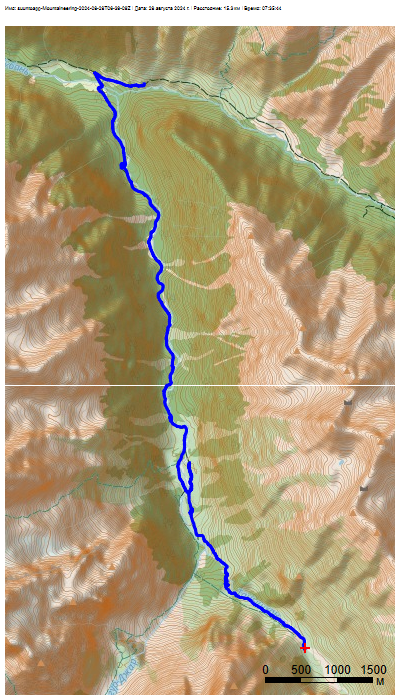
\includegraphics[angle=0, width=0.3\linewidth]{../pics/mini_maps/28}
	\label{fig:mini_28}
\end{figure}

*воспоминания вики: проснулись, пошли по кустарникам вдоль реки, вышли к мужикам, гоняющим коровок, вдоль накатанной дороги и по цивильным мостам дошли до места стоянки*

=======
*воспоминания вики: проснулись, пошли по кустарникам вдоль реки, вышли к мужикам, гоняющим коровок, вдоль накатанной дороги и по цивильным мостам дошли до места стоянки*
Просто текст cyjdf ghjcnj vkege
>>>>>>> 45e3ec5fb9d7c526ee62dbc08bdd583692404d5d
\newpage